\chapter{Data}
\label{ch:dataset}

\glsreset{mimiciii}

In this chapter, we describe the dataset used in our study and outline the data preparation steps undertaken to support our analysis. We discuss the structure of the dataset, the types of data it contains, and the specific tables utilized for extracting relevant information. Understanding the dataset intricacies is crucial for replicating our work and ensuring the validity of our findings.

\section{Dataset Description}
\label{sec:dataset-description}


The \gls{mimiciii} version 1.4  is a large, publicly available database comprising deidentified health-related data associated with \num{\TotalPatients} patients who were admitted to critical care units at the Beth Israel Deaconess Medical Center in Boston, Massachusetts, between 2001 and 2012 \cite{MIMICIII}. The database includes comprehensive clinical data collected during routine hospital care, supporting reproducible research, and fostering advancements in critical care medicine.

Data access is provided through PhysioNet \cite{PhysioNet} following completion of the ``CITI Data or Specimens Only Research'' course and signing of the data use agreement. The dataset was downloaded from Google Cloud on 2024-07-20.

The \gls{mimiciii} database integrates data from:

\begin{itemize}
    \item Archives from critical care information systems
    \item Hospital electronic health records
    \item The Social Security Administration Death Master File
\end{itemize}

Two different critical care information systems were used during the data collection period: \emph{Philips CareVue Clinical Information System} and \emph{iMDsoft MetaVision ICU}.

Prior to inclusion in the \gls{mimiciii} database, data were deidentified in accordance with \gls{hipaa} standards using structured data cleansing and date shifting. The deidentification process involved the removal of all eighteen identifying data elements specified by \gls{hipaa}, including patient names, telephone numbers, addresses, and dates. The dates were shifted to preserve the intervals, resulting in hospital stays that appeared between the years 2100 and 2200. The time of day, day of the week, and approximate seasonality were maintained during date shifting. For patients older than 89 years, the dates of birth were shifted to obscure their true age, resulting in recorded ages of over 300 years in the database.

The project was approved by the Institutional Review Boards of Beth Israel Deaconess Medical Center and the Massachusetts Institute of Technology. The requirement for individual patient consent was waived because the project did not affect clinical care and all protected health information was deidentified.

\section{Data Structure and Usage}
\label{sec:data-structure}

The \gls{mimiciii} database consists of 26 relational tables. Charted events, such as physiological measurements, laboratory tests, and fluid balances, are stored in tables ending with \texttt{\_EVENTS}. For instance, the \texttt{CHARTEVENTS} table contains time-stamped observations recorded by nurses and clinical staff, while the \texttt{LABEVENTS} table contains laboratory test results.

Tables prefixed with \texttt{D\_} are dictionary tables that provide definitions for the identifiers used in the events tables. For example, \texttt{CHARTEVENTS} is associated with \texttt{D\_ITEMS}, which provides descriptions of the measured concepts. By joining \texttt{CHARTEVENTS} and \texttt{D\_ITEMS} on the \texttt{ITEMID} column, one can identify the meaning of a given \texttt{ITEMID}.

The tables used in this study include:

\begin{itemize}
    \item \texttt{CHARTEVENTS}: Charted events, such as physiological measurements and observations;
    \item \texttt{INPUTEVENTS\_CV} and \texttt{INPUTEVENTS\_MV}: Input events (e.g., medications and fluids administered) from the CareVue and MetaVision systems, respectively;
    \item \texttt{LABEVENTS}: Laboratory test results;
    \item \texttt{OUTPUTEVENTS}: Measurements related to patient outputs (e.g., urine output);
    \item \texttt{D\_ITEMS} and \texttt{D\_LABITEMS}: Dictionary tables providing item definitions;
    \item \texttt{ADMISSIONS} and \texttt{PATIENTS}: Demographic and admission information;
    \item \texttt{ICUSTAYS}: \gls{icu} stay information, including mortality outcomes.
\end{itemize}

The data from all these tables were merged and processed to construct a unified dataset suitable for analysis, involving joins on relevant keys, alignment of time-stamped events, and consolidation of measurements from different sources.

\section{Cohort and Feature Selection}

In this study, we selected only adult patients aged 18 years or older. For the unsupervised value forecasting task described in \cref{sec:pretraining}, we included data from all \gls{icu} stays that meet this criterion. For the supervised mortality prediction task described in \cref{sec:finetuning}, we further restricted the dataset to \gls{icu} stays where the patient survived for at least \num{24} hours. We aim to predict in-hospital mortality using data from the first \num{24} hours of the \gls{icu} stay. In the selected cohort, the prevalence of in-hospital mortality is \num{\DeathPrevalence}.

The raw number of unique measurement types (the number of rows in \texttt{D\_ITEMS} and \texttt{D\_LABITEMS}) in the \gls{mimiciii} database is \num{\NumberOfRawFeatures}, with many referring to similar clinical variables that reflect the same biological processes. For instance, there are six distinct items representing ``Glucose (Blood)'', each having a unique identifier in the observation tables. These variations can refer to different measurement methods, such as fingerstick or laboratory analysis, or originate from different systems (CareVue and MetaVision).

Following the data processing pipeline described by \textcite{STraTS2022}, we extracted \num{\NumberOfFeatures} features corresponding to different clinical variables. Each feature was manually selected and grouped by their corresponding identifiers to ensure consistency. This grouping ensured that all observations related to the same biological process were accurately combined, despite differences in measurement methods or originating systems. Measurements recorded in different units were converted to common units to maintain uniformity across the dataset. In addition, we include demographic information (age and gender) as features to provide context for clinical data.

In \cref{fig:hist_glucose_blood}, the stacked histograms of blood glucose measurements show similar distributions across pooled observations. This kind of visual validation was conducted for every selected feature to confirm that the grouped observations represent the same underlying biological phenomena.

\begin{figure}
    \centering
    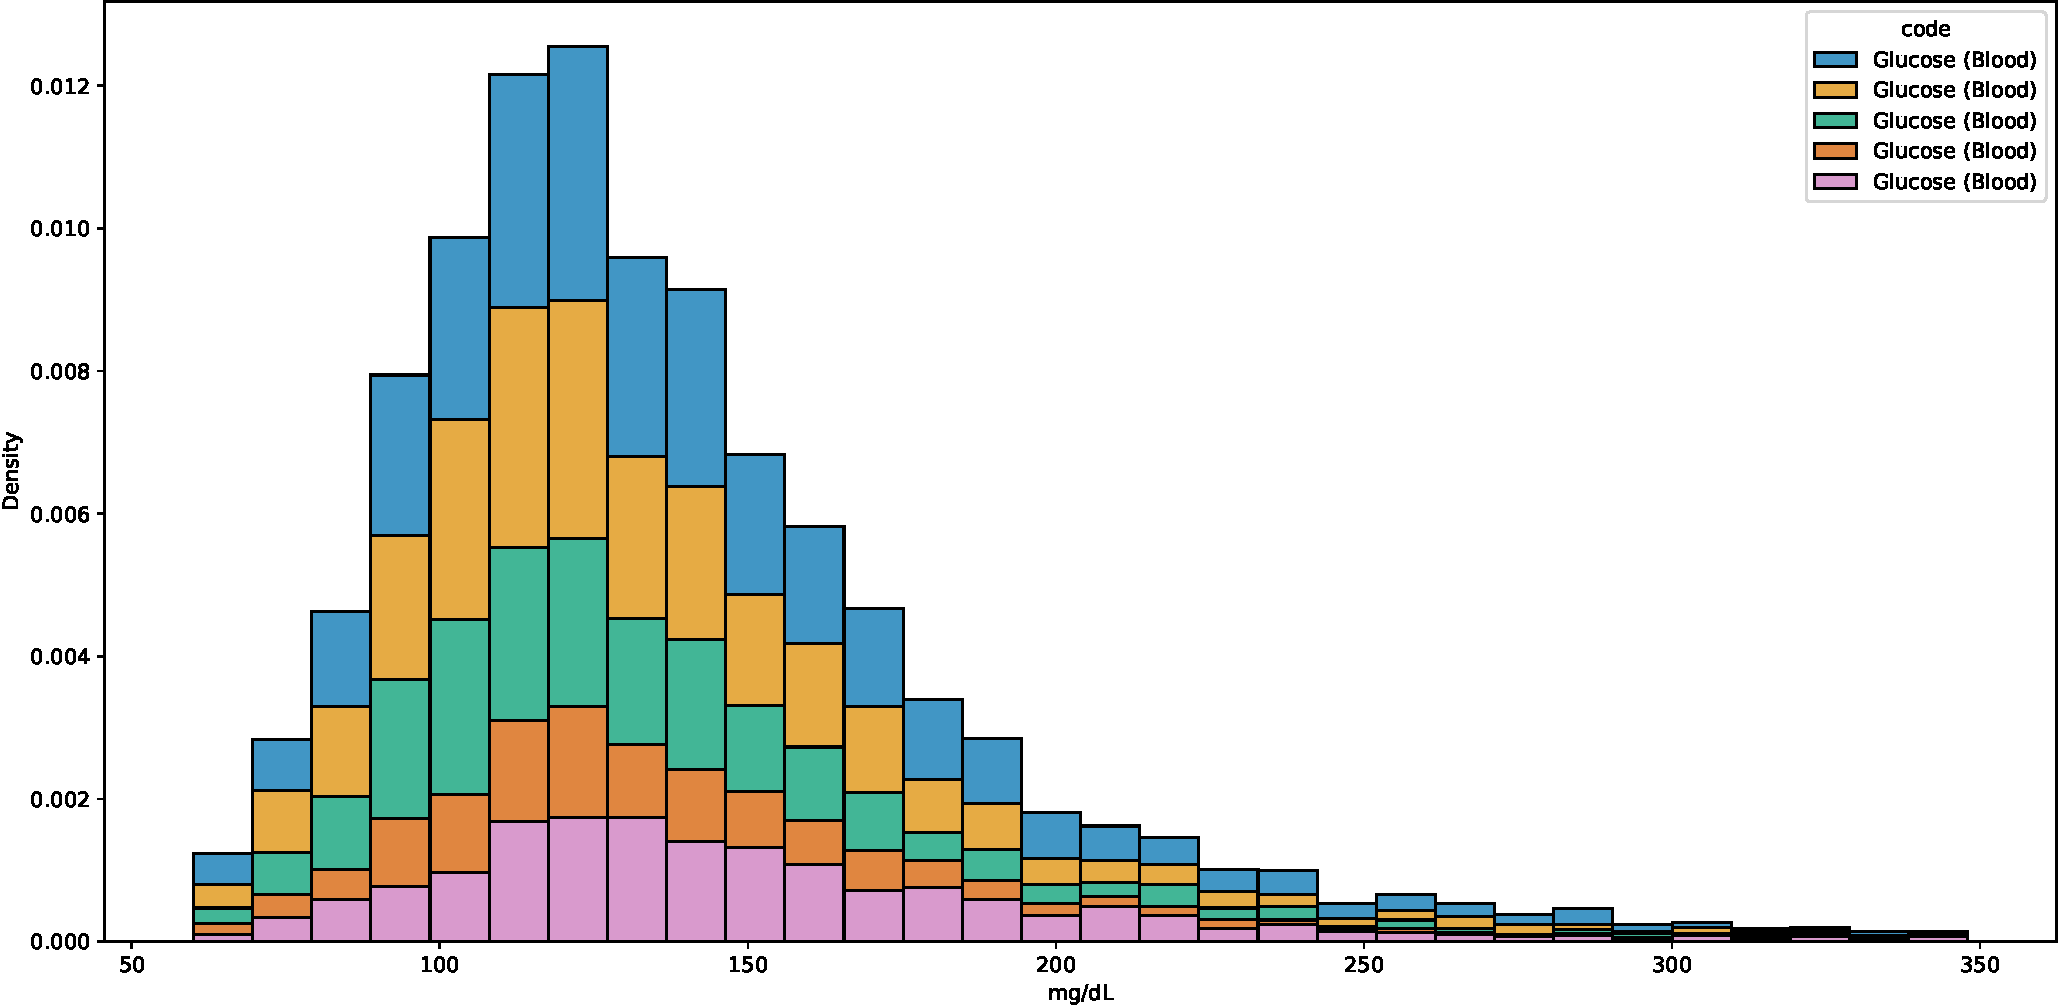
\includegraphics[width=\textwidth]{./figures/hist_Glucose}
    \caption{Distribution of blood glucose values}
    \label{fig:hist_glucose_blood}
\end{figure}

\section{Outlier Processing}
\label{sec:outlier-processing}
Following the methodology described in the original paper, outliers were handled using different strategies based on the type of the event. For each feature, boundaries of valid values were manually defined based on medical expertise and clinical guidelines. Values outside these ranges were identified as outliers and processed accordingly:

\begin{itemize}
    \item \emph{Input and Output Events:} Outliers were replaced with the median value of the respective feature. This approach mitigates the influence of extreme values while preserving the central tendency of the data.
    \item \emph{Chart and Lab Events:} Outliers in these events were removed from the dataset, ensuring analyses were not skewed by erroneous or implausible measurements.
\end{itemize}

Defining valid ranges based on medical knowledge ensured that the outlier detection process was grounded in clinical relevance. For example, physiological measurements that fall outside humanly possible ranges (e.g., a heart rate exceeding \qty{390}{\text{bpm}} or a negative blood pressure) were flagged as outliers.


\section{Value Distributions}

To determine appropriate normalization techniques and understand the characteristics of our data, we analyzed the distributions of the selected features.

Using common normality tests, such as Shapiro-Wilk and Kolmogorov-Smirnov, did not provide satisfactory results due to the large number of observations, which led to extremely small p-values, sometimes beyond \texttt{float32} precision. Therefore, we opted for visual inspection of the distributions and computed skewness ($\gamma$) and excess kurtosis ($\kappa$), as well as the Wasserstein distance ($d_w$) between the Z-transformed observed data and a standard normal distribution. This approach allowed us to identify notable deviations from normality and assess the need for alternative normalization techniques.

Specifically, only \num{25} out of \num{129} features (\qty{19.4}{\percent}) demonstrated relatively low Wasserstein distance from a normal distribution ($d_w < 0.2$), only \num{20} features (\qty{15.5}{\percent}) had low skewness ($|\gamma| < 1$) and only \num{8} (\qty{6.2}{\percent}) had low excess kurtosis (\(|\kappa| < 1 \)). High absolute skewness and high kurtosis indicate asymmetric distributions and heavy tails, which can adversely affect algorithms sensitive to extreme values or non-normality. This motivated us to explore alternative normalization techniques that do not rely on the normality assumption. A detailed statistics for all selected features can be found in \cref{ch:features_statistics}.


\section{Feature Correlations}

Analyzing feature correlations aids in identifying relationships within the dataset, informing feature selection, and guiding model development. Correlation analysis can reveal multicollinearity, where two or more features are highly correlated, which may affect the performance of certain models. It also provides insights into potential dimensionality reduction and reflects underlying biological processes.

Spearman's \( \rho \), a rank correlation coefficient, was used due to the skewed nature of many feature distributions. Spearman's correlation provides a more suitable analysis as it measures the strength and direction of monotonic (but not necessarily linear) relationships between features, making it robust to non-normal distributions and less sensitive to extreme values.

The correlation matrix in \cref{fig:correlation_matrix}, providing an overview of the \num{50} features with highest absolute Spearman's correlations, reveals clusters of highly correlated features. For example, levels of direct, indirect, and total bilirubin are strongly correlated, suggesting they reflect related physiological processes. However, most features exhibit low absolute correlation coefficients, indicating that the selected features provide largely unique information, thus avoiding redundancy. The low absolute rank correlations suggest that capturing relationships between features may require modeling nonlinear and complex interactions, highlighting the potential benefit of advanced modeling techniques.

\begin{figure}
    \centering
    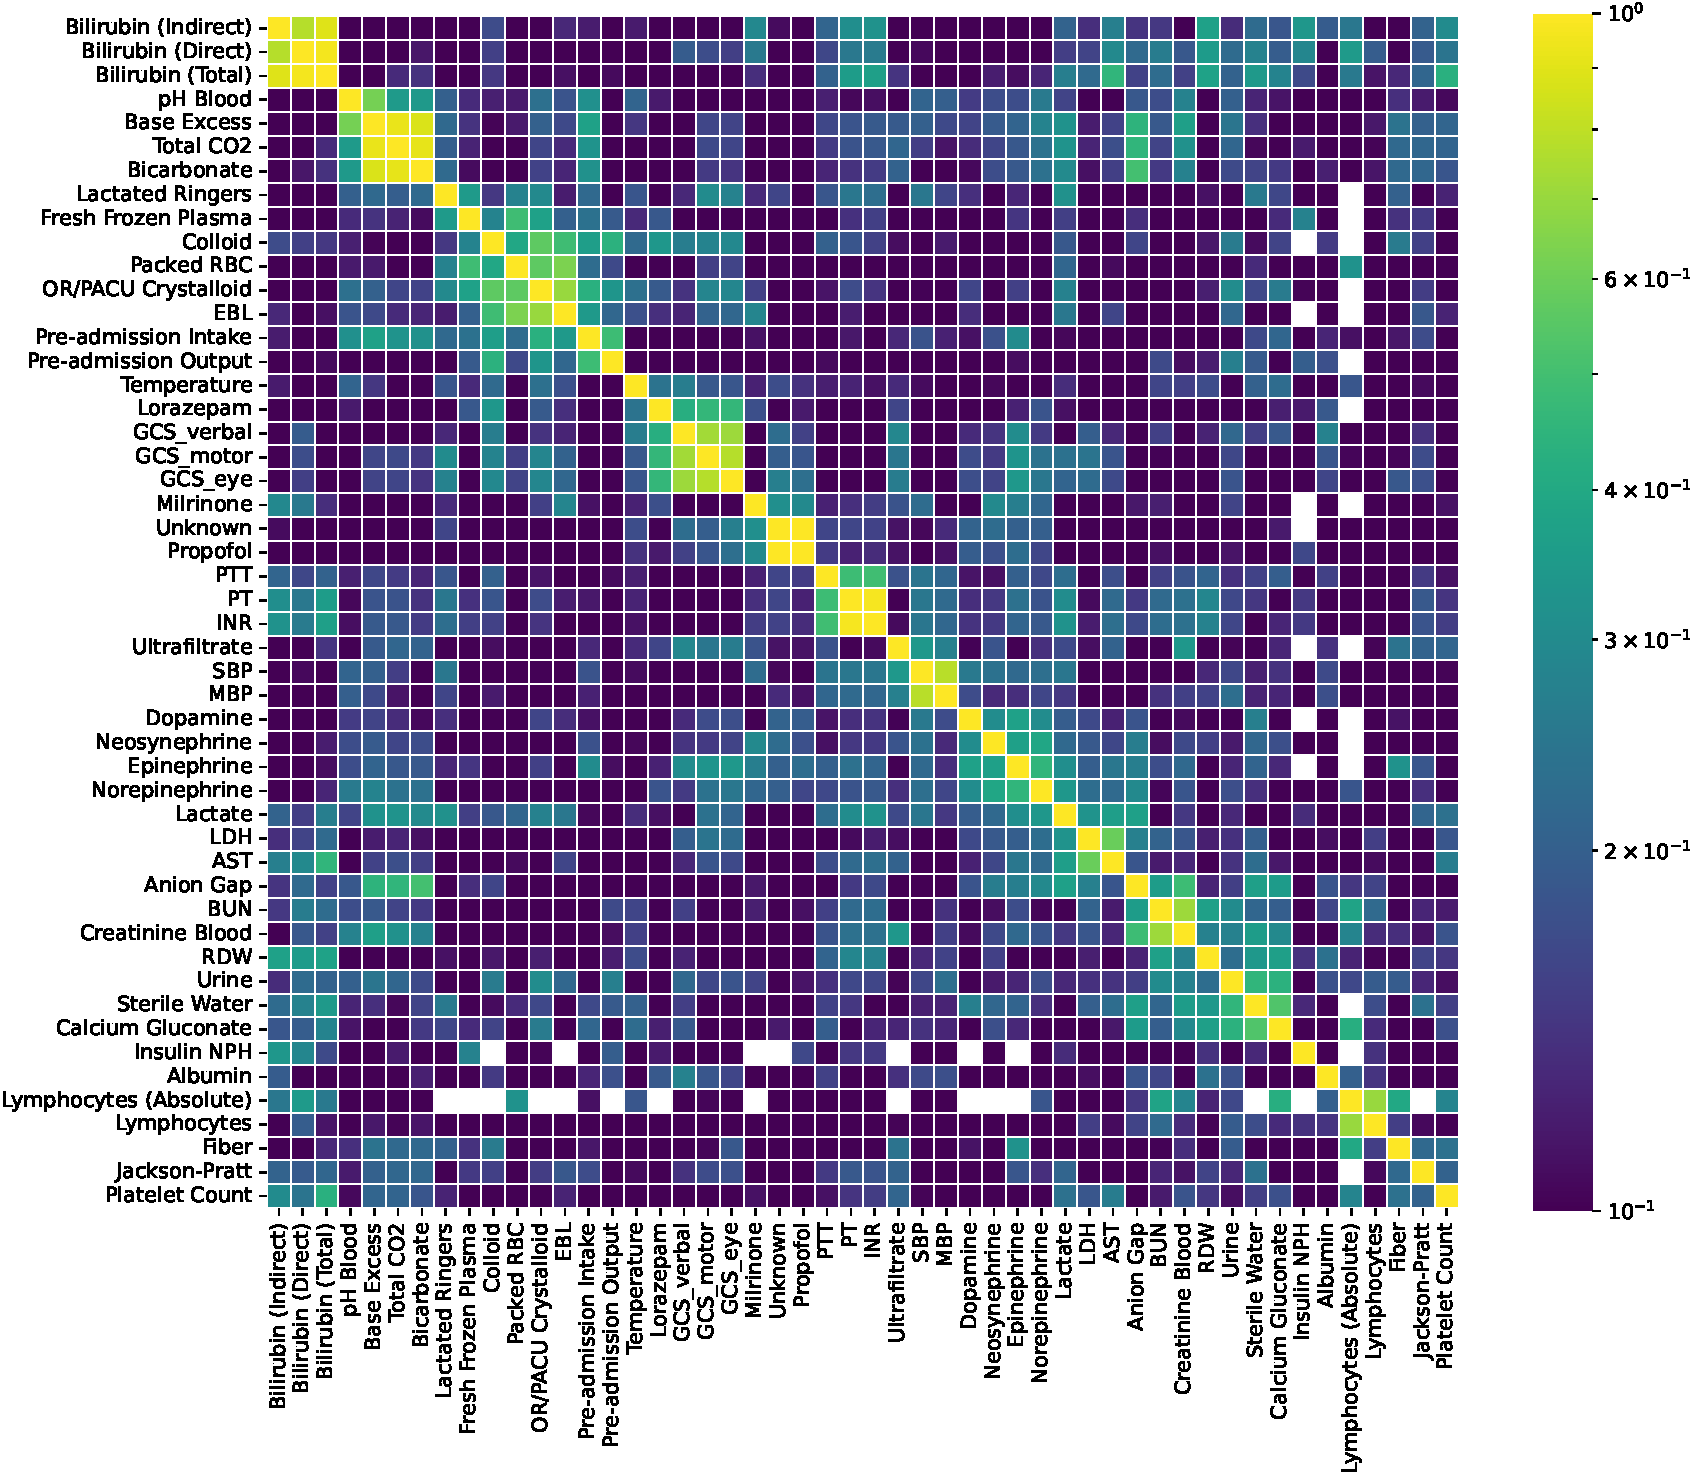
\includegraphics[width=\textwidth]{./figures/correlation_matrix}
    \caption[Spearman $\rho$]{Within-day absolute Spearman correlation of the 50 most correlated features}
    \label{fig:correlation_matrix}
\end{figure}


\section{Patient's Journey Visualizations}

\Cref{fig:journey_292741} illustrates a multivariate clinical time series consisting of \num{\patientJourneyShortLength} observations with irregular time points for a single patient. The Viridis color map indicates the relative value of each measurement compared to other measurements of the same type across the entire dataset, with dark blue representing the lowest values and yellow representing the highest values. To enhance visualization and prevent overlapping, measurements that occur within short time intervals are depicted with smaller circles.

The patient's journey shown in \cref{fig:journey_292741} has fewer observations than the average \gls{icu} stay. On average, an \gls{icu} stay contains \num{1822(4275)} events. For comparison, \cref{ch:patient_journey} presents a visualization of a patient journey with a higher number of measurements.

\begin{figure}
    \centering
    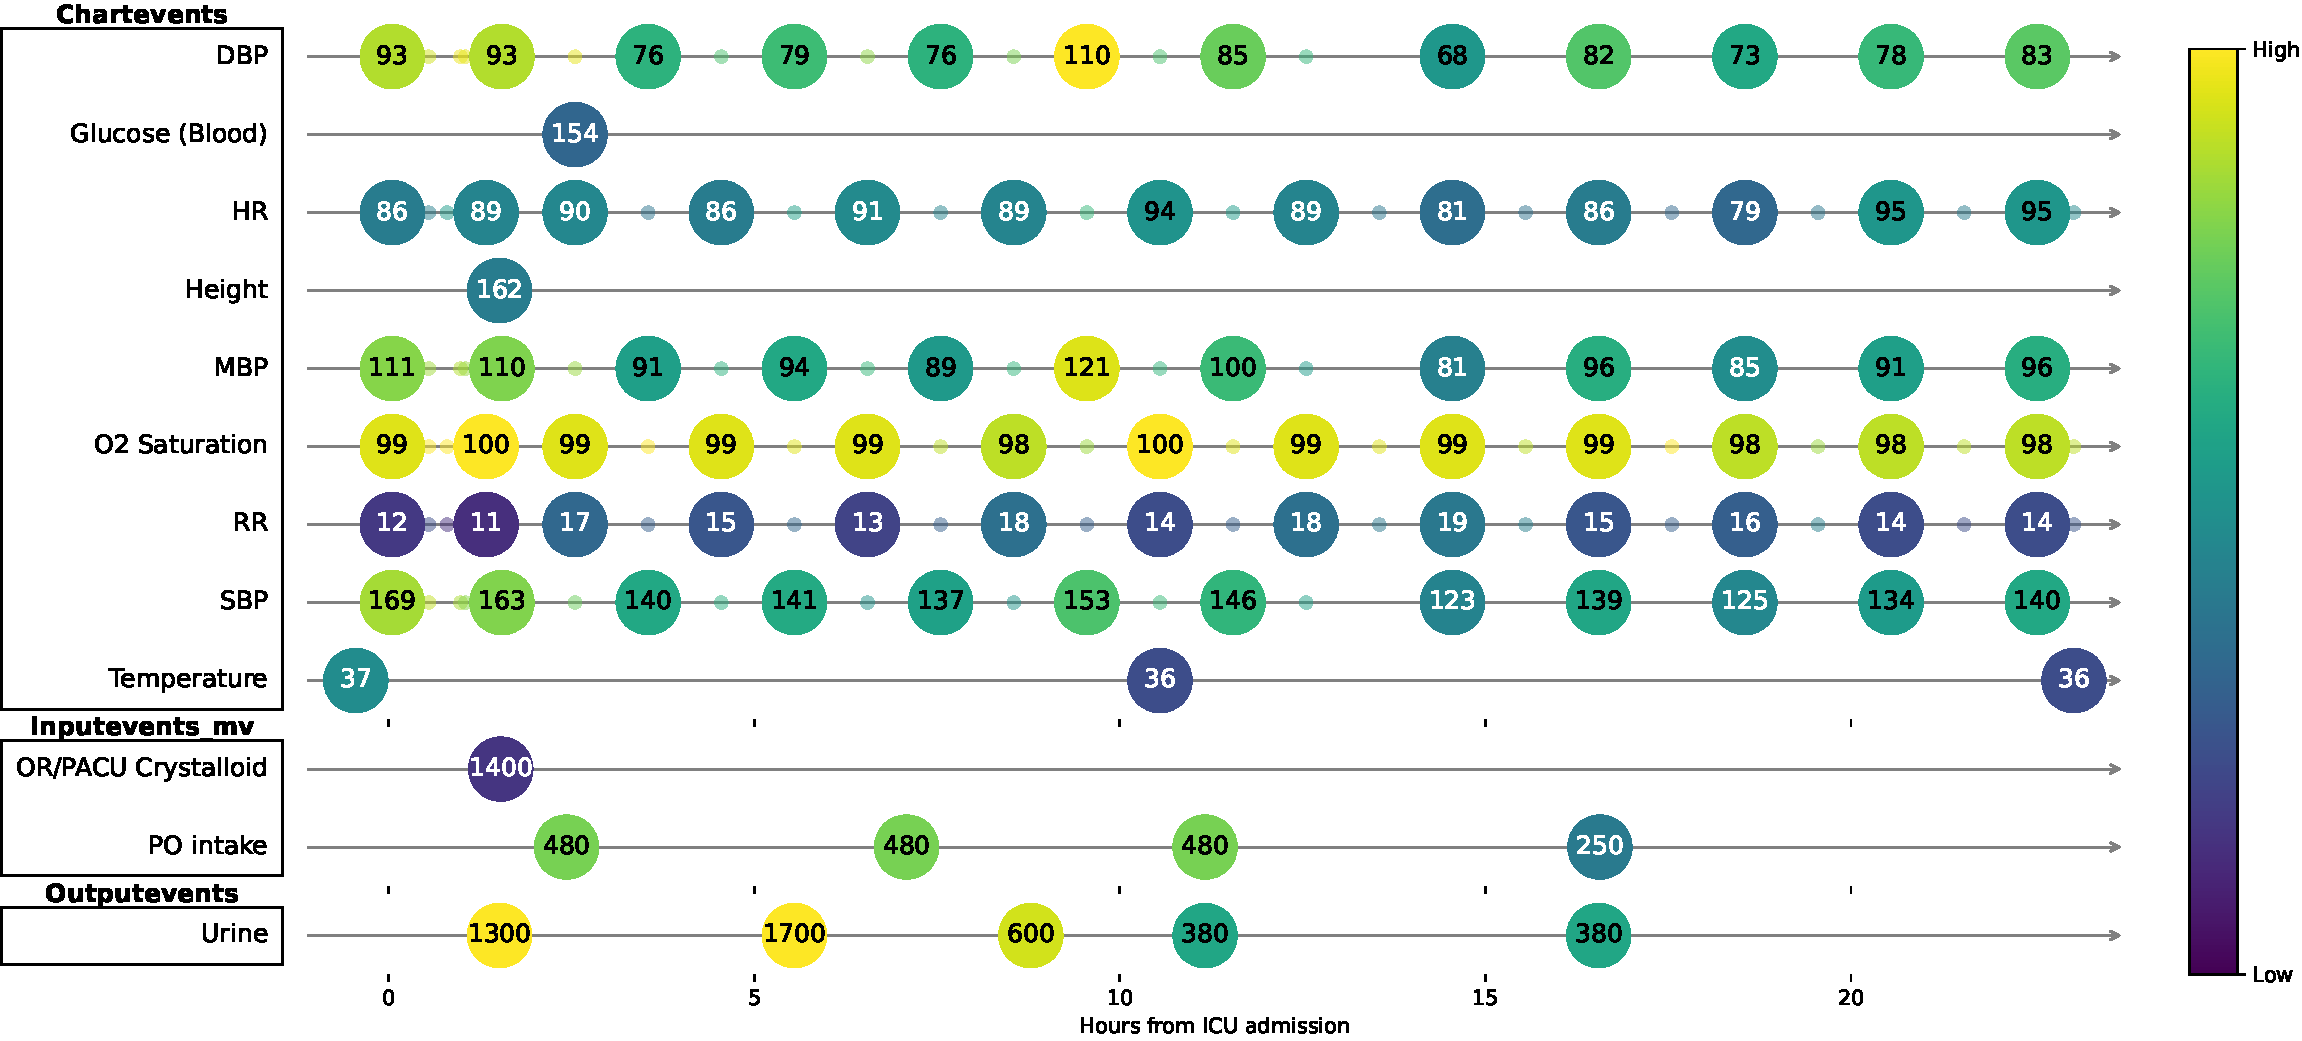
\includegraphics[height=\textheight, width=\textwidth, keepaspectratio]{./figures/journey_292741}
    \caption{Visualization of a multivariate clinical time series with irregular time points and missing values for a single patient}
    \label{fig:journey_292741}
\end{figure}

These visualizations highlight common challenges in clinical health data:

\begin{itemize}
    \item \textbf{Missingness and Sparsity}: Not all features are observed for all patients due to varying clinical needs. As a result, the time-series data are sparse, with some features measured more frequently than others.
    \item \textbf{Irregular Time Intervals}: Clinical measurements are not always taken at regular intervals. The timing of measurements depends on the patient's condition and clinical decisions, leading to sporadic data collection.
\end{itemize}

These challenges complicate data analysis and model development. The handling of missing data and irregular sampling requires advanced methods capable of capturing the temporal dynamics and relationships within the data despite its sparsity and irregularity.


\section{Technical Details of Data Processing}

\subsection{Data Splitting}

To evaluate the generalization capability of the model and prevent data leakage between sets, the dataset was divided into training, validation, and test splits at the patient level \cite{emmert2019evaluation}. The data for each patient are contained entirely within one subset, maintaining the integrity of the evaluation. This patient-level splitting strategy ensures unbiased and reliable performance metrics, providing a solid foundation for model evaluation and comparison.

Following the approach described by \textcite{STraTS2022}, the labeled data were split into a 64:16:20 ratio:

\begin{itemize}
    \item \textbf{Training set} (\qty{64}{\percent}): Used to fit the model's parameters.
    \item \textbf{Validation set} (\qty{16}{\percent}): Used to evaluate model performance during training.
    \item \textbf{Test set} (\qty{20}{\percent}): Reserved for the final evaluation of the model's performance on unseen data.
\end{itemize}

\Cref{tab:split_statistics} presents the distribution of the number of patients in each set.

\begin{table}[h!]
    \centering
    \caption{Statistics of the dataset splits}
    \label{tab:split_statistics}
    \begin{tabular}{lrrr}
\toprule
Split & Number of events & Number of patients & Number of ICU stays \\
\midrule
Unsupervised train & 51,497,384 & 27,289 & 36,849 \\
Supervised train & 49,478,011 & 21,372 & 28,790 \\
Test & 14,886,798 & 6,679 & 8,878 \\
Validation & 11,951,075 & 5,344 & 7,144 \\
\bottomrule
\end{tabular}

\end{table}

\subsection{Data Processing Tools and Technologies}

The data processing pipeline was implemented using Apache Spark \cite{ApacheSpark} and orchestrated with Snakemake \cite{SnakeMake}. This combination allowed for efficient handling of large datasets and reproducible workflow management.

\subsubsection{Apache Spark for Data Processing}

The original data processing pipeline provided by the original paper relied on the Pandas Python library, which required loading the entire dataset into RAM. Due to the large size of the dataset, this approach resulted in excessive memory consumption, causing the Python process to terminate after exhausting \qty{50}{\giga\byte} of RAM (including \qty{20}{\giga\byte} of swap memory).

To address this limitation, the data processing code was rewritten using Apache Spark \cite{ApacheSpark}. Spark's distributed computing capabilities allowed for efficient data processing without the need to load the entire dataset into memory.

Each table of the dataset is provided as a separate CSV file, and collectively they occupy  \qty{39}{\giga\byte} of disk space. The files were converted into a set of Parquet files to enable faster processing and simplify the analysis. The Spark-based pipeline processed the Parquet dataset, utilizing all available \num{16} CPU threads and \qty{16}{\giga\byte} of RAM at peak load, and completed the processing in \qty{5(1)}{\minute}. This represents an order of magnitude speed improvement compared to the original Pandas-based pipeline, which took \qty{53}{\minute} (as was consequently measured after increasing the available RAM to accommodate the process).

Although rewriting the data processing code in Spark provided practical experience and significant performance gains, it required substantial effort and increased the complexity of the codebase. In situations where development time is limited, an alternative approach could be to utilize a cloud virtual machine with more RAM and employ a simpler Pandas-based pipeline if the budget allows.

\subsubsection{Workflow Management with Snakemake}

We used Snakemake to orchestrate all data processing steps. Snakemake is a workflow management system that enables reproducible and scalable execution of complex data workflows. It ensures that each step of the data processing pipeline is executed in the correct order and that dependencies are properly managed, facilitating the reproducibility of the experiments.

\section{Chapter Conclusion}

This chapter has detailed the dataset used in the study, including its structure, the cohort and feature selection process, and the challenges associated with clinical time-series data. The data processing techniques employed, including the use of Apache Spark and Snakemake, were instrumental in efficiently handling the large and complex dataset. Understanding these technical details is crucial for replicating the study and provides a foundation for the modeling approaches discussed in the following chapters.

